% !TEX root=../../Thesis.tex
\chapter{Introduction} \label{ch:intro}
The way we transport ourselves is currently evolving, and \gls{ad} technology is expected to have a big impact on this transformation~\cite{traffic21, McKinsey2023}. With \gls{av} the efficiency of traffic can be improved by scheduling commercial transports outside of rush hours~\cite{FAGNANT2015167}. The number of parking spots in cities can be reduced if the vehicles can autonomously drive itself to a less crowded area when not in use and drive back when needed. Congestion and traffic jams could also be reduced if a large amount of vehicles in traffic are autonomous and optimize around the same goal e.g., traffic flow or fuel efficiency. 

The rapid success of \gls{ml} during the last decades has lead to major progress towards deploying \gls{av}s in the real world. One clear benefactor of these new \gls{ml} techniques are the perception systems~\cite{Janai2020}. Better perception enables more accurate representation of the environment. 
% The low-level control of the vehicle is a mature research area and can be solved with classical control theory methods~\cite{Paden2016}.
However, navigating complex scenarios such as urban intersections and roundabouts with dense traffic remain challenging for \gls{av}s because it requires a higher level of interaction between road users, as summarized in a review paper~\cite{Schwarting2018}. 
When human drivers approach an intersection, they normally assess who has the right of way, before deciding whether to proceed or yield to other road users. However, human drivers do not always follow the rules.
% When a human drivers approach an intersection, they observe the environment to identify the traffic light, signs and other approaching vehicles. Then assess the situation to determine \textit{who has the right of way?} Before deciding weather to drive or yield. 
% If all drivers could perfectly assess the situation and follow the right of way, there would be no accidents or collisions between cars. 
% Despite, each year over one million people are killed in traffic-related accidents, where the vast majority of the accidents are caused by human mistakes~\cite{WHO2018, NHTSA2018}. 
According to the Insurance Institute for Highway Safety~\cite{IIHS2019}, in 2019, an estimated \num{115741} people were injured by drivers running a red light, whereas \num{928} of them were killed. 
While these accidents were mainly caused by driver inattention or reckless driving, it motivates the development of decision-making algorithms for \gls{av}s which not only follow the traffic rules but can also take into account other drivers future actions and inattention, which is the main focus in this thesis. 
%\todo{Level 2: Volvo pilot assist and tesla auto pilot. Level 4: Waymo. Woven automated city}
% That is why this thesis will focus on intersection scenarios that includes interactions of other vehicles and propose a \gls{rl} approach using deep Q-learning while considering the uncertainty of . 

% This thesis presents a deep Q-learning approach for creating decision-making strategies for \gls{av}s driving in environments with other drivers without explicitly knowing their intentions. 
% Starting with introducing the different \gls{ad} levels in Section~\ref{sec:intro_ad}.
% Section~\ref{sec:intro_intersections} defines the terms' scenario, intersection and intention used in this thesis.
% \Citet{Shalev2016} raises two concerns when using \gls{ml}, especially Reinforcement learning, for autonomous driving applications: ensuring functional safety of the driving policy and solving the \gls{mdp} model is problematic, because of unpredictable behavior of other drivers. 
% Ensuring functional safety is not the main focus of this work, but because of its importance, it is briefly addressed in Section~\ref{sec:system_architecture} together with a proposed system architecture that can utilize the work presented in this thesis in a ''safe'' way. 
% The handling of the unpredictable behavior of other drivers is the main topic in this thesis and the research questions are presented in Section~\ref{sec:research_questions}. The scope and limitations are listed in Section~\ref{sec:scope}. Finally, the contributions of this thesis is presented in Section~\ref{sec:contributions}. 

\section{Autonomous Driving Levels}
\label{sec:intro_ad}
% \tommy{I would start with one or two sentences introducing the problem. Saying that the thesis deals with intersections, and that's interesting because this and that (maybe super challenging, accidents, interactive situations, not sure what's best to mention). And the go into the details of how you define intersection, intention, and scenario.}
When talking about autonomous driving, it is first important to specify which level of autonomy that is being discussed. The Society of Automotive Engineers has classified these different levels of autonomy ranging from zero to five~\cite{SAE2021}, also referred to as L0-L5. The first level L0 is a vehicle with no autonomy, whereas a fully \gls{av} that can operate in any environment and without any human supervision is defined as L5. Popular \gls{adas} functions today, like lane centering or adaptive cruise control are classified as L1, while the Volvo Pilot Assist and Tesla Autopilot that provide both steering and acceleration/braking are classified as level 2. The main criteria for L2 systems is that the driver is in control and only supported by the system. This puts a requirement on the driver to always supervise the vehicle and take over when needed to ensure safety. For L3 and higher the responsibility of driving is shifted to the system. At L3, the driver still has to take control over the vehicle but at only the request of the system, and at L4 and L5 the autonomous driving features no longer require the driver to take over. Finally, the main difference between L4 and L5 is the capability of driving anywhere, under all conditions. Examples of L4 are robot taxis developed by Waymo, Zoox, cruise and Toyota which only operate in a specified area or city. 

% Another way to categorize these autonomy levels is: supervised and unsupervised driving. Supervised driving include L0-L3 where the driver has to supervise the system and take control when necessary, while unsupervised 

The \gls{av} making the decisions in this work are referred to as the ego vehicle, while other traffic participants are assumed to be vehicles driven by other human drivers but could be extended to pedestrians bicyclist and other \gls{av}s. 
The methods presented in this thesis are aimed at an autonomy level L3-L5. At the highest level the system is expected to handle all aspects of driving within a specific task such as crossing an intersection at any location. 


\section{Intersections, intention and scenarios}
\label{sec:intro_intersections}
When it comes to the scenarios considered in this work. This section aims to clarify the use of the words' intersection, intention and scenario.
% When a pedestrian approach a crossing they have been taught at a young age to look at both sides of the road before crossing. The same apply for a human driver approaching an intersection. 
% When a human driver approach an intersection, it is natural to observe the environment to identify the traffic light, signs and other approaching vehicles. Then assess the situation, who has the right of way? 

% The intention of the other driver can be guided by the 
% Recently nontraditional intersections are also becoming increasingly popular. The goal of these designs is to reduce the number and/or severity of conflict points by altering the customary vehicular paths at the intersection. In light of the increased focus on and occurrence of these intersection types, it is expected that the application of nontraditional designs will continue to spread.

\begin{figure}[h]
	\centering
	\begin{subfigure}[t]{0.48\columnwidth}
		\centering
		\begin{tikzpicture}
			% Crossing
			\def\crossleftx{-2}
			\def\crossrightx{2}
			\def\crosstopy{2}
			\def\crossboty{-2}
			\def\roadwidth{0.5}

			\draw (0,0) circle (2pt);
			\node at (1.2, 0.2) {conflict point};
			\draw[thick] (\crossleftx, \roadwidth) -- (-\roadwidth, \roadwidth) -- (-\roadwidth, \crosstopy);
			\draw[thick] (\crossleftx, -\roadwidth) -- (-\roadwidth, -\roadwidth) -- (-\roadwidth-\roadwidth, \crossboty);
			\draw[thick] (\roadwidth, \crosstopy) -- (\roadwidth, \roadwidth) -- (\crossrightx, \roadwidth);
			\draw[thick] (\roadwidth-\roadwidth, \crossboty) -- (\roadwidth, -\roadwidth) -- (\crossrightx, -\roadwidth);

			% 	cars
			\node[inner sep=0pt] (ego_car) at (\crossleftx+0.5,0)
			{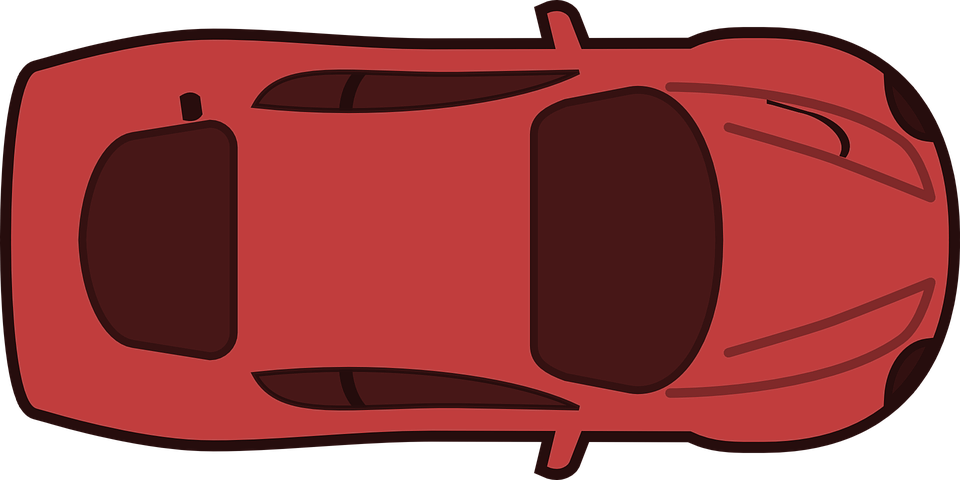
\includegraphics[width=.18\textwidth, angle=0]{figures/ego_car_top_down.png}};

			\node[inner sep=0pt] (target_car) at (0,\crosstopy-0.5)
			{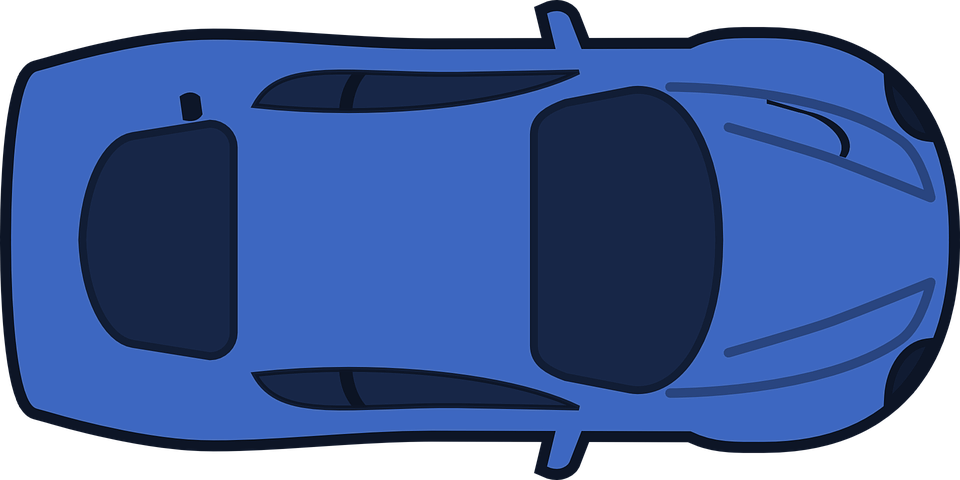
\includegraphics[width=.18\textwidth, angle=-90]{figures/target_car_top_down.png}};

			\node[inner sep=0pt] (target_car) at (-.1,-0.8)
			{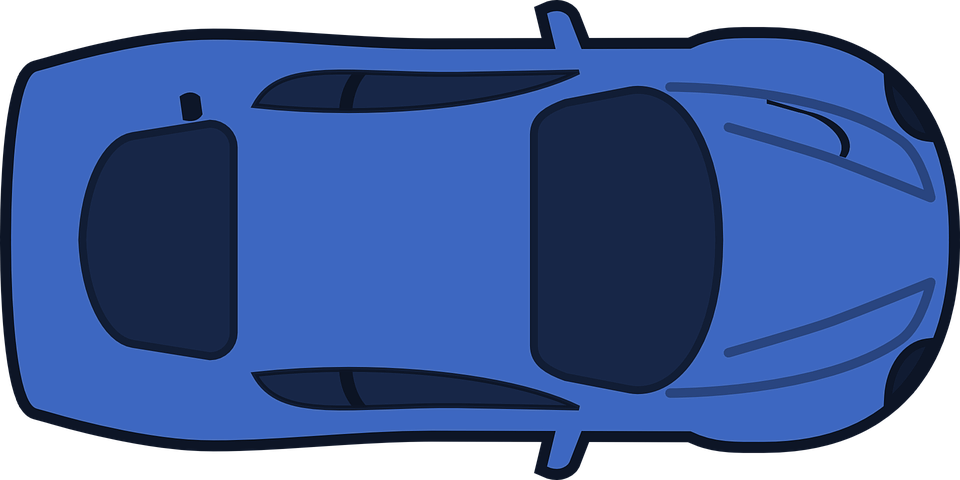
\includegraphics[width=.18\textwidth, angle=-110]{figures/target_car_top_down.png}};


		\end{tikzpicture}
		\caption{Single intersection}
\end{subfigure}%
	~ 
	\begin{subfigure}[t]{0.48\columnwidth}
		\centering
		\begin{tikzpicture}
			% Crossing
			\def\crossleftx{-2.5}
			\def\crossrightx{2.5}
			\def\crosstopy{2}
			\def\crossboty{-2}
			\def\roadwidth{0.5}

			\draw (-0.5,0) circle (2pt);
			\draw (0.5,0) circle (2pt);
			% \node at (0.7, 0.2) {crossing point$^1$};
			\draw[thick] (\crossleftx, \roadwidth) -- (-\roadwidth-0.5, \roadwidth) -- (-\roadwidth-0.5, \crosstopy);
			\draw[thick] (\crossleftx, -\roadwidth) -- (-\roadwidth-0.5, -\roadwidth) -- (-\roadwidth-0.5, \crossboty);
			\draw[thick] (0, \crosstopy) -- (0, \roadwidth);
			\draw[thick] (0, -\roadwidth) -- (0, \crossboty);
			\draw[thick] (\roadwidth+0.5, \crosstopy) -- (\roadwidth+0.5, \roadwidth) -- (\crossrightx, \roadwidth);
			\draw[thick] (\roadwidth+0.5, \crossboty) -- (\roadwidth+0.5, -\roadwidth) -- (\crossrightx, -\roadwidth);

			% 	cars
			\node[inner sep=0pt] (ego_car) at (\crossleftx+0.5,0)
			{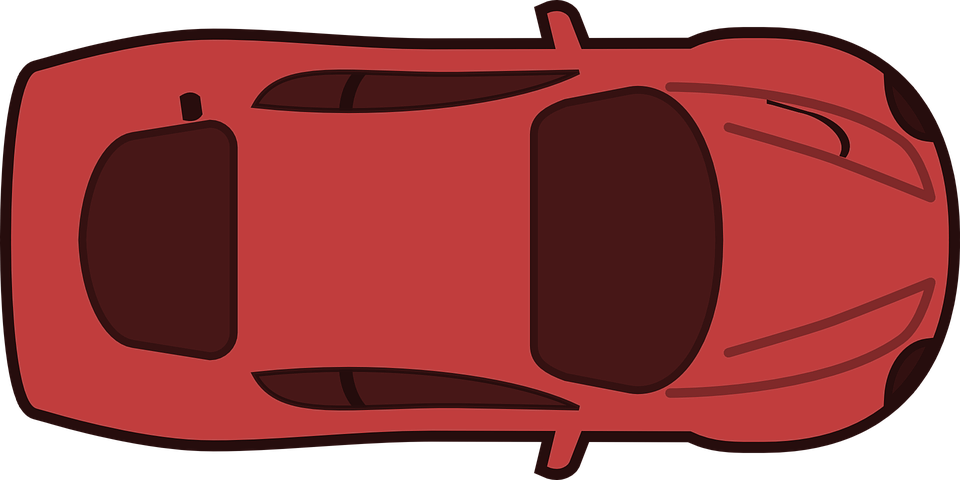
\includegraphics[width=.18\textwidth, angle=0]{figures/ego_car_top_down.png}};

			\node[inner sep=0pt] (target_car) at (-0.5,\crosstopy-0.5) {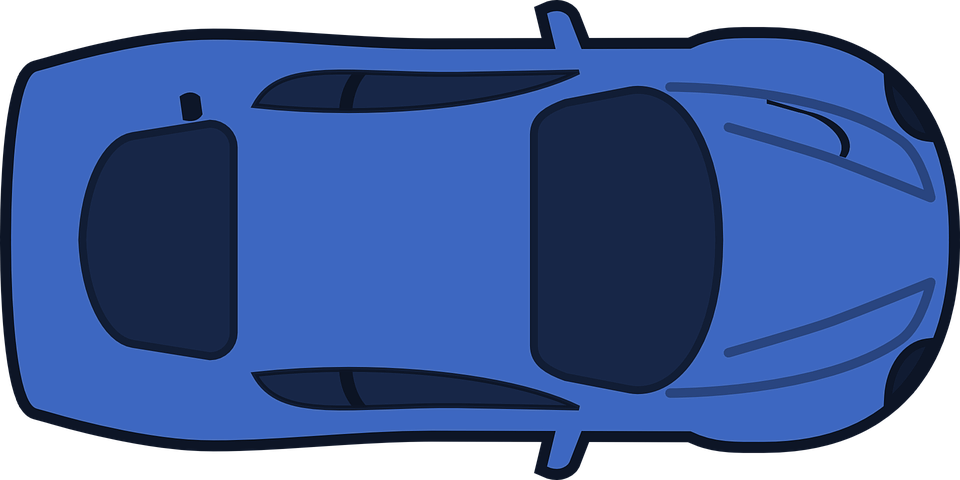
\includegraphics[width=.18\textwidth, angle=-90]{figures/target_car_top_down.png}};

			\node[inner sep=0pt] (target_car_2) at (0.5,\crossboty+0.5) {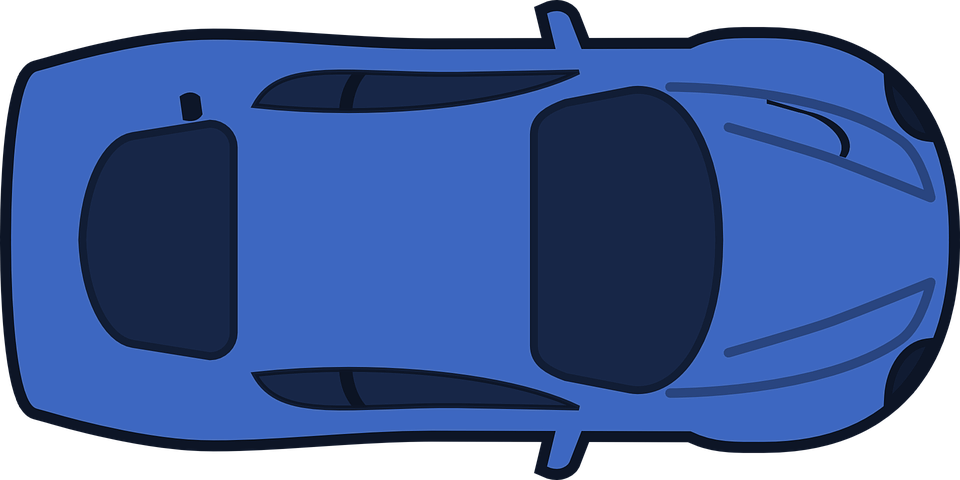
\includegraphics[width=.18\textwidth, angle=90]{figures/target_car_top_down.png}};

		\end{tikzpicture}
		\caption{Double intersection}
	\end{subfigure}

	\caption{Examples of different intersections}
	\label{fig:example_intersections}
\end{figure}
Let's begin by defining the terms 'intersection,' 'intention,' and 'scenario' within the context of this study.
An intersection refers to the geometric layout of roads intersecting each other, encompassing elements such as the number of junctions, conflict points, turns, and angles of incidence, as illustrated in Figure~\ref{fig:example_intersections}. 
Intersections can be categorized as signalized or unsignalized. A signalized intersection is equipped with mechanisms to designate the right-of-way, such as regulatory signs (e.g., STOP or YIELD) or traffic signals, while an unsignalized intersection lacks such features. However, as emphasized in the introduction, human drivers do not always adhere strictly to these right-of-way rules, which can result in accidents. Therefore, this thesis defines intentions as the anticipated actions of other vehicles in the future, such as stopping, cautiously slowing down, or proceeding through the intersection.

\begin{figure}[h]
	% \mbox{\parbox{\textwidth}{
	% \centering
	% % \vspace{0.3cm}
	% 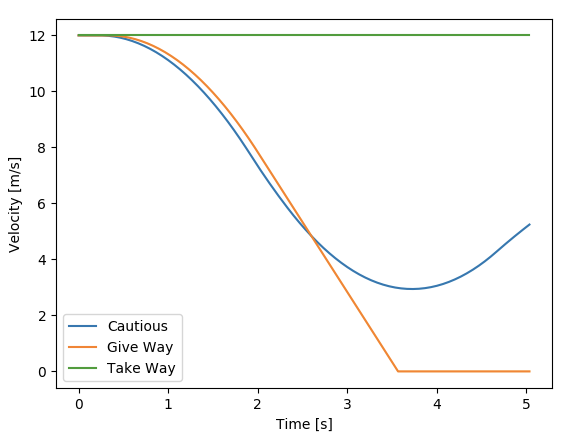
\includegraphics[width=0.6\columnwidth]{YourThesis/papers/mpc/figures/velocity_profiles_agents.png}
	% }}
	\centering
	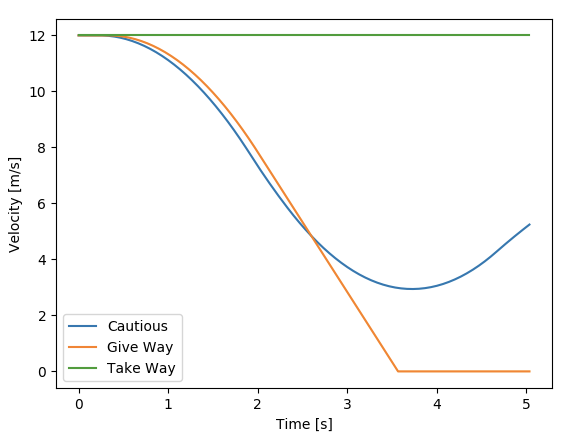
\includegraphics[width=0.6\columnwidth]{YourThesis/papers/mpc/figures/velocity_profiles_agents.png}

	\caption{An illustration showing velocity profiles for agents with three distinct intentions. Each agent shares the same initial position and velocity while approaching a common intersection.}
	\label{fig:intro_intention_profiles}
	% \vspace{-0.3cm}
\end{figure}

Figure \ref{fig:intro_intention_profiles} illustrates how velocity profiles can differ for three different intentions. In this example, distinguishing between the 'give way' and 'take way' intentions is straightforward, as the velocity begins to decelerate at time $0$. However, identifying the 'cautious' intention poses a challenge, as the agent cannot be certain until the other vehicle comes to a complete stop.

If intentions are known, intersections can be treated as unsignalized, as the right-of-way can be inferred from the intentions rather than relying solely on infrastructure. This approach ensures safety even in situations where another vehicle disregards traffic rules, such as running a red light, as a cautious agent will prioritize safety and stop accordingly.

\section{The intersection problem}
\begin{figure}
	\mbox{\parbox{\textwidth}{
		\centering
		\begin{tikzpicture}
			\def\xstart{-7};

			\coordinate (p) at (3,0);
			\foreach \n/\w/\c in {z0/2/green,z1/2/red,z2/2.5/orange,z3/3.5/blue}{
				\node[rectangle,
				draw=none,
				anchor=east,
				text = black,
				fill = \c!60,
				minimum width = \w cm, 
				minimum height = 2cm] 
				(n) at (p) {\Huge \n};
				
				\coordinate (p) at (n.west);
			}

			% Crossing
			\draw[line width=0.5mm] (\xstart, 1) -- (-1, 1) -- (-1, 5);
			\draw[line width=0.5mm] (\xstart, -1) -- (-1, -1) -- (-1, -2);
			\draw[line width=0.5mm] (1, 5) -- (1, 1) -- (3, 1);
			\draw[line width=0.5mm] (1, -2) -- (1, -1) -- (3, -1);
			
			% cars
			\node[inner sep=0pt] (ego_car) at (-7,0)
			{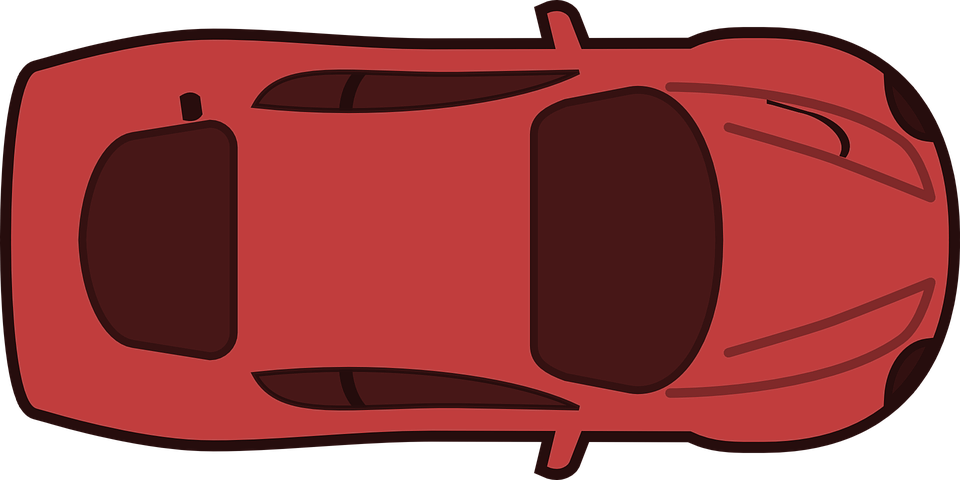
\includegraphics[width=.18\textwidth, angle=0]{figures/ego_car_top_down.png}};
			\node[inner sep=0pt] (target_car) at (0,4)
			{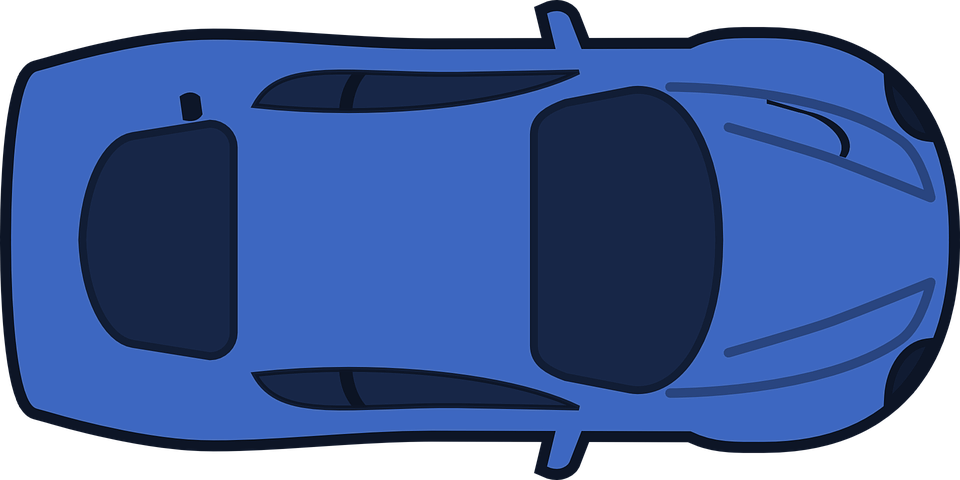
\includegraphics[width=.18\textwidth, angle=-90]{figures/target_car_top_down.png}};

	\end{tikzpicture}
	}}
	\caption{Intersection scenario divided into zones describing what is required of the decision maker in different zones}
	\label{fig:zones}
\end{figure}

With the \gls{mdp} defined, the path of the ego vehicle can be segmented into four zones as shown in Figure~\ref{fig:zones}. Starting from the end, Zone 0 represents the 'safe zone,' where the ego vehicle is out of danger and can resume nominal driving. Zone 1 is the 'conflict zone,' where a collision with another vehicle is possible. Zone 2, the 'critical decision zone,' is the final opportunity for the vehicle to either stop or proceed through the intersection. The size of zone 2 is determined by the minimum distance required for the vehicle to come to a complete stop before entering the conflict zone, ensuring sufficient time for safe decision-making. Lastly, Zone 3, the 'information gathering zone,' is situated furthest from the intersection. Here, the agent can observe how other vehicles behave over time to estimate their intentions.

The goal is to reach Zone 0. To achieve this, the agent aims to minimize the time spent in Zone 1 if there is a chance of intersection with another car. Our actions are formulated as short-term goals, designed for comfortable use with lower acceleration rates. The size of Zone 2 depends on the vehicle's current speed, which is influenced by its behavior in Zone 3.

Now, two conflicting strategies emerge: to minimize time in Zone 1, the agent desires a high speed entering the intersection. However, it also seeks a low speed to reduce the size of Zone 2 and the critical decision period. If the intentions of other vehicles are known, the stochasticity in Zone 1 would be eliminated, transforming the problem into a scheduling task aimed at creating a velocity profile that minimizes the time required to cross. However, since the intentions of other vehicles are stochastic, reinforcement learning offers a promising approach to address this uncertainty and optimize decision-making in dynamic traffic scenarios.


\section{Research questions}
\label{sec:research_questions}
% This thesis defines human driving as sequential decision making under uncertainty. Decisions such as overtaking a slow driver or when to cross an intersection are often made with limited information and some prediction estimate based on previous experience. 
% This section briefly introduce the intersection problem, why its hard and the research questions that are studied in this paper. 
% % A simple unsignalized intersection is shown in Figure \ref{fig:zones}.
% In some cases like highway driving the uncertainty is very low, but when it comes to more urban environment this uncertainty increases. Compared to highway, urban environments introduce more uncertainty. 
% Investigate how \gls{rl} methods can be used in practice to create a tactical decision making agent for \gls{ad}.


% \begin{enumerate}
% 	\item The goal for the ego vehicle is to drive through intersections without colliding. 
% 	\item The intersection can be of different shapes. %We assume we have a map of the intersection. 
% 	\item There will be other vehicles crossing the same intersection. 
% 	\item The intention of other drivers are not known
	
% \end{enumerate}

This thesis focuses on investigating and evaluating \gls{rl} agents for navigating complex intersection scenarios, with a particular emphasis on managing uncertainty. 
The intersection navigation problem is formulated as a \gls{pomdp}, where observable states include positions and velocities of vehicles, while unobservable states pertain to the intentions of surrounding drivers. These following research questions are considered:

\begin{enumerate}
	\item[\textbf{Q1.}] How can \gls{rl} techniques be used to develop a decision-making agent that effectively navigates intersections without explicitly estimating the intention state of other vehicles?
\end{enumerate}
% To answer this, a deep Q-learning approach is employed to solve the POMDP, using short-term goals as actions. These short-term goals are translated into reference points and constraints for a controller. Specifically, Paper A utilizes a sliding mode controller, while Paper B employs \gls{mpc}.
A deep Q-learning approach is used to solve the \gls{pomdp}, with short-term goal as actions. These short-term goals are translated into references points and constraints for a controller. \paperLSTM \ uses a sliding mode controller, while \paperMPC \ uses a \gls{mpc}.
To address the challenge of unobservable intentions, the hidden state in the \gls{lstm} layer of the \gls{rl} agent is designed to incorporate estimations of these intentions, crucial for informed decision-making in dynamic traffic environments. 

\begin{enumerate}
	\item[\textbf{Q2.}] How can an \gls{rl} agent utilize the uncertainty in its predictions and actions to enhance decision-making in complex environments? 
\end{enumerate}
Two main sources of uncertainty are tackled in this thesis: Q-value uncertainty and intention state uncertainty.
For Q-value uncertainty, \paperEnsamble \ estimates the uncertainty in the Q-values predicted by using an ensemble of neural networks on different subsets of the available data. This ensemble provides a distribution over the estimated $Q$-values and the uncertainty in choosing different actions can be defined as the coefficient of variation of the $Q$-values.
% the \gls{dqn} and applies a confidence criterion to avoid risky actions. 
In \paperBelief, the hidden intention states of other vehicles are represented using a belief state generated via a particle filter. This belief state provides a probability distribution over possible true states, which informs the agent's decisions.

Two methods are proposed to handle intention estimation: QMDP-IE and QID. QMDP-IE, derived from the QMDP algorithm, uses a single estimated intention state, reducing computational complexity while blending elements of POMDPs and MDPs. In contrast, QID represents the intention state using a belief state distribution, allowing for more adaptive and robust decision-making in uncertain environments.

\begin{enumerate}
	\item[\textbf{Q3.}] How can an \gls{rl} agent handle situations it has not been trained on? 
\end{enumerate}
A confidence criterion is applied to the uncertainty of the estimated $Q$-values in \paperEnsamble, making actions with high uncertainty invalid and if no action satisfies the confidence criterion a backup action e.g., emergency breaking, can be applied avoiding potential collisions. If the uncertainty measure from \paperEnsamble \ and \paperBelief \ can be used to identify that the agent is in the wrong environment, the transfer \gls{rl} approach from \paperTransfer can be employed to determine which environment out of a set of environments the agent is currently in, or to select the policy that best fits the current situation
% The developed algorithms are evaluated in both trained and untrained scenarios. Detailed collision analyses are conducted to identify failure points in the agent's decision-making process. The performance of QMDP-IE and QID is compared against baseline algorithms (QMDP and QPF) to assess their effectiveness in reducing collisions and handling untrained scenarios. The results indicate that QID is better at handling scenarios outside the training set by taking passive actions that can alter the intention distribution and reduce uncertainty in subsequent states. Meanwhile, QMDP-IE offers a structured approach with moderate collision rates and higher computational efficiency.



% The work presented in this thesis investigate the following research questions:
% \begin{enumerate}
% 	\item[\textbf{Q1.}] How can \gls{rl} techniques be used to develop a decision-making agent that effectively navigates intersections without explicitly estimating the intention state of other vehicles? (PAPER A and B)
% 	\item[\textbf{Q2.}] How can an \gls{rl} agent utilize the uncertainty in its predictions and actions to enhance decision-making in complex environments? (PAPER C and D)
% 	\item[\textbf{Q3.}] How can an \gls{rl} agent handle situations it has not been trained on? (PAPER C and E)
	
% 	% \item[\textbf{Q3.}] How can the quality of a RL agent be improved by accounting for uncertainty? (PAPER C and D)
% 	% \item[\textbf{Q1.}] How can RL be used to create a decision-making agent for autonomous driving, that can handle different unsignalized intersections (complex urban scenarios)? Learn a scalable policy that is able to handle different scenarios. Relative coordinate system. Action space. 
% 	% (specificera for att komma undan varfor har du inte kollat pa andra metoder. How can we use RL for AD )
% 	% \item[\textbf{Q2.}] Can a good driving policy be found without explicitly predicting other drivers intentions?
% 	% \item[\textbf{Q2.}] Can we find a driving policy without explicitly predicting other drivers intentions?
% 	% LSTM or other netowrk structures can find the hidden state that is intention. 
% 	% \item[\textbf{Q3.}] How can MPC be used to improve the action and state space for a RL agent? 
% 	% \item[\textbf{Q3.}] How do we model the actions to drive through an intersection as discreet? (PAPER A and B)
% 	% \item[\textbf{Q3.}] How can AD domain knowledge (and models) be used to improve the action and state space for a RL agent? MPC for actions, Particle filter for intention distribution. How can AD domain knowledge be used to create a state and action space that improves the RL agent?
% 	% (How can the uncertainty of the RL agent be utilized?) (RPF-in the output and PF-in the input space)
% 	% \item[\textbf{Q5.}] Where does ML/RL fit in the system architecure for decision making?
% 	% (PAPER A shows that RL can make decisions that finds a gap inbetween cars, PAPER B found that we RL can learn the utility of different actions and decrease the computational power required by modeling and predicting each action in the MPC. While MPC can ganerate a safe path that guarantees safety.) 
% \end{enumerate}

\section{Scope and limitations}
\label{sec:scope}
The following aspects of creating a tactical decision-making agent for autonomous driving in uncertain environments are not considered in this thesis. 

\begin{enumerate}
	% \item We have access to sensors on-board the ego vehicle. We do not have v2v, or v2x communication. 
	% \item We do not assume any knowledge of traffic signs or traffic lights. 
	% \item Do not guarantee safety, the best we can do its making the decisions not trigger collision avoidance functions. 
	\item Guaranteeing safety in \gls{ad} systems is an important open question that is out of scope for this thesis. 
	\item The work in this thesis is tested in simulation environments and not real world. 
	\item This work considers the control of one vehicle and not multiple agents. 
	% \item Although there are many interesting \gls{rl} algorithms out there, this work is only focused on deep Q-learning. 
	% \item This work considers the control of one vehicle and not multiple agents. 
	% \item A reward function is defined for each approach. 
	
	% To compensate for not having v2v or v2x communication, we have to, directly or indirectly, predict what other driver will do. 
	
\end{enumerate}


\section{Contributions}
\label{sec:contributions}
% \todo{Rewrite once thesis is in a better state}
The main contributions of this thesis are:
\begin{enumerate}
	\item A deep Q-learning approach for creating a decision-making agent navigating intersection that considers the intentions of other drivers. 
	% \item A \gls{pomdp} formulation for driving in intersections. 
	\item A neural network architecture that is invariant to permutations of the order of which surrounding traffic participants are observed, which speeds up training and improves the quality of the trained agent. 
	\item A belief state representation of driver intentions using a particle filter.
	\item A belief state \gls{dqn} method that can adjust the aggressiveness of the policy using one threshold parameter.
	% \item Two approached to solving a \gls{pomdp} with hidden intention state. LSTM layer and belief state. 
	% \item General state space representation that is invariat to permutations of the intersection design. 
	\item Extension of \gls{rl} methods that provide an uncertainty estimate of the proposed decisions and use it to create a confidence criterion that can identify situations with high uncertainty. 
	% \item Method for choosing between a set of fully trained policies. 
	\item A transfer learning method that is able to identify the which \gls{mdp} the agent is in, out of a set of \gls{mdp}s.
\end{enumerate}


\section{Thesis outline}
% \todo{rewrite when thesis is more finished}
The outline of the thesis is as follows: in Chapter \ref{ch:related_work} other research in the same field is presented. In Chapter \ref{ch:background} introduce the mathematical framework \gls{mdp} and \gls{pomdp} with a brief theory of \gls{rl}, deep Q-learning and the \gls{idm}. 
Chapter \ref{ch:modeling_intersection} is where the problem is formulated by defining the components of the \gls{pomdp}. Results from using deep Q-learning to solve the \gls{pomdp} is presented and later combined with a \gls{mpc} to improve the actions. Later in Chapter \ref{ch:uncertainty} two approaches to handle the uncertainty is presented. First the uncertainty in the decisions from the \gls{rl} algorithm and then an empirical study of how well a \gls{dqn} can handle uncertainty of others driving intentions. Chapter \ref{ch:generalize} present an approach to generalize over different \gls{mdp}s more specifically policies learned from different transfer functions. Finally, Chapter \ref{ch:conclusion}provides some concluding remarks. 
% \todo{add discussion, conclusions and included papers}

